\subsection{Classification at the normative limits}

Table~\ref{tab:trees} reports the out-of-fold metrics of the binomial trees. The 2 [mpy] tree reached a mean recall of 0.710 (0.646 for the non-exceeding class, 0.774 for the exceeding class) and the 8 [mpy] tree reached 0.808 with a recall ratio of 0.986. Both trees exceed the acceptance threshold of 0.6 with balanced per-class sensitivity. Figure~\ref{fig:cm} shows the three-class confusion matrix composed from the two out-of-fold binary decisions: the strategy recovers 0.60, 0.47, and 0.75 of the low, medium, and high classes, with the adjacent medium class as the hardest region.

\begin{table}[htb!]
\centering
\footnotesize
\setlength{\tabcolsep}{4pt}
\caption{Binomial decision trees at the normative limits: out-of-fold metrics of the nested cross-validation (Mean: mean per-class recall; Ratio: min/max recall).}
\label{tab:trees}
\begin{tabular}{@{}cccccc@{}}
\toprule
Limit & Mean & Ratio & Recall$_{\leq}$ & Recall$_{>}$ & Acc. \\
\midrule
\midrule
2 [mpy] & 0.710 & 0.834 & 0.646 & 0.774 & 0.742 \\
8 [mpy] & 0.808 & 0.986 & 0.803 & 0.814 & 0.807 \\
\bottomrule
\end{tabular}
\end{table}


\begin{figure}[htb!]
  \centering
  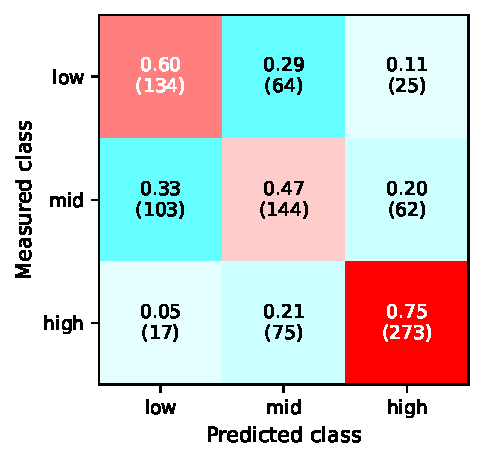
\includegraphics[width=0.62\linewidth]{figures/confusion_matrix.pdf}
  \caption{Three-class out-of-fold confusion matrix (row-normalized; record counts in parentheses).}
  \label{fig:cm}
\end{figure}

Figure~\ref{fig:trees} presents the deployed trees. Both organize the fleet by its service history and geometry: the 2 [mpy] tree separates the monitoring regime by service time, flow velocity, and gas rate, and the 8 [mpy] tree isolates the severe regime among the young, small-diameter, gas-rich lines.

\begin{figure*}[htb!]
  \centering
  \begin{subfigure}{0.85\textwidth}
    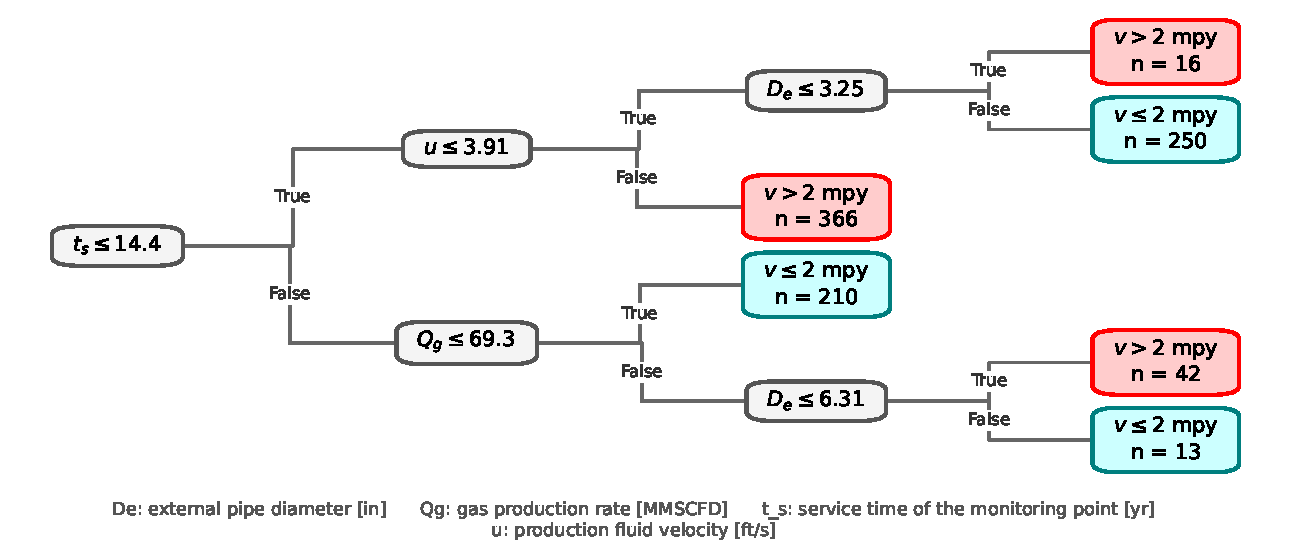
\includegraphics[width=\linewidth]{figures/tree_th2.pdf}
    \caption{}
  \end{subfigure}
  \begin{subfigure}{0.95\textwidth}
    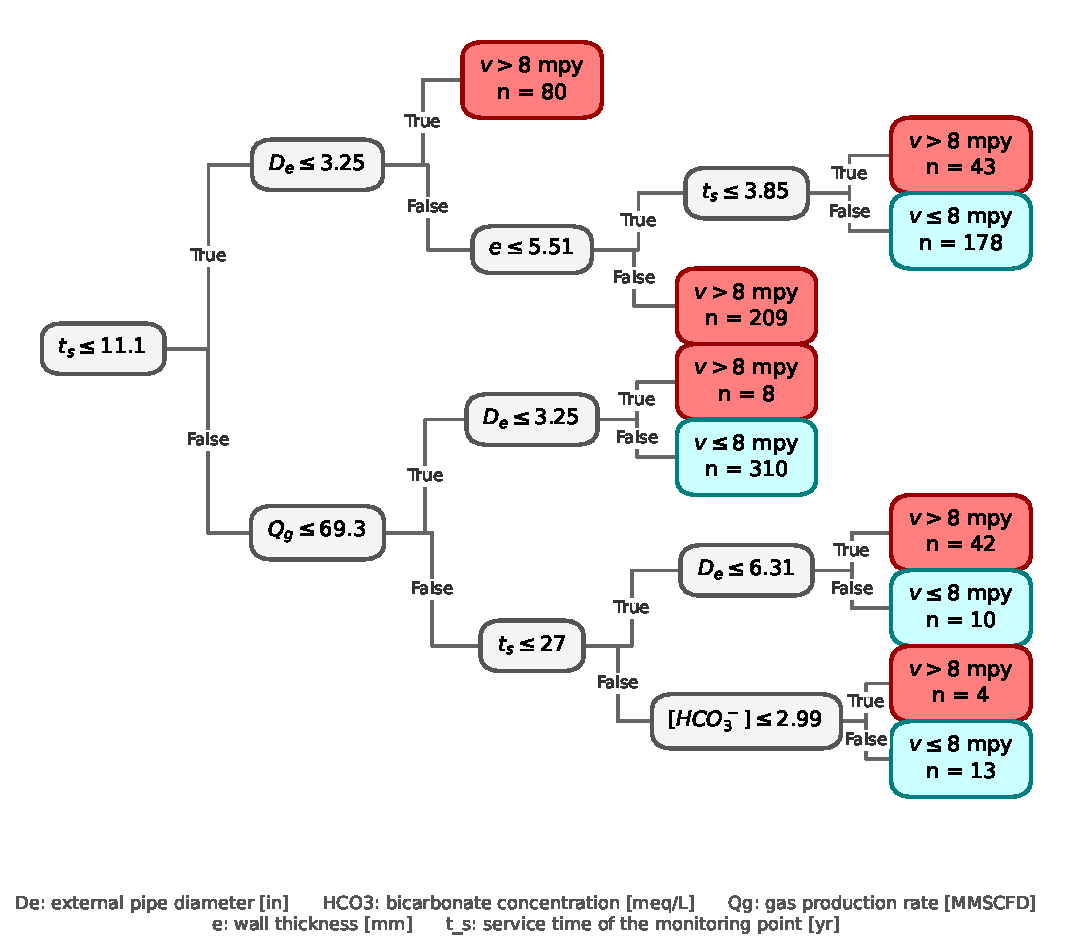
\includegraphics[width=\linewidth]{figures/tree_th8.pdf}
    \caption{}
  \end{subfigure}
  \caption{Deployed binomial trees after merging the partitions that do not change the decision: (a) 2 [mpy] limit, (b) 8 [mpy] limit. Teal leaves do not exceed the limit; red leaves exceed it; $n$ is the number of training records per leaf.}
  \label{fig:trees}
\end{figure*}

\subsection{Deployed rulebase and physical reading}

The full-data refit produced twelve rules over six variables: the service time $t_s$, the fluid velocity $u$, the external diameter $D_e$, the gas rate $Q_g$, the wall thickness $e$, and the bicarbonate concentration $[\mathrm{HCO_3^-}]$ (Table~\ref{tab:rules}). Figure~\ref{fig:coverage} quantifies the share of the output that each rule carries within its own severity zone. The rules organize the asset population by its service history and duty:

\begin{itemize}
  \item \textbf{R1} (low, $c_1 = 2.0$ [mpy]): young lines ($t_s \leq 14$ [yr]) of larger diameter ($D_e > 3.25$ [in]) under slow flow ($u \leq 3.9$ [ft/s]): low wall shear on a large section keeps the attack inside the monitoring range.
  \item \textbf{R2} (low, $c_2 = 1.2$ [mpy]): mature lines ($t_s > 14$ [yr]) with low gas rate ($Q_g \leq 69$ [MMSCFD]). This is the dominant low rule (46\% of the zone): a line that has survived beyond fourteen years under quiet service demonstrates a benign environment, and the low gas rate limits turbulence and CO$_2$ supply.
  \item \textbf{R3} (low, $c_3 = 2.0$): mature lines with high gas rate but large diameter ($D_e > 6.3$ [in]): the section area keeps the mixture velocity, and with it the wall shear, low.
  \item \textbf{R4} (mid, $c_4 = 7.1$): young, slow, small-diameter lines. The ordinal exclusion suppresses this rule completely (0\% contribution): its region belongs to the severe rule R7, which demonstrates the exclusion operating as designed.
  \item \textbf{R5} (mid, $c_5 = 6.0$): young lines under fast flow ($u > 3.9$ [ft/s]): flow-enhanced attack before any protective layer consolidates. Dominant medium rule (22\% of the zone).
  \item \textbf{R6} (mid, $c_6 = 6.2$): mature, gas-rich lines of small diameter: the sustained turbulence keeps the rate in the intensified-inspection range.
  \item \textbf{R7} (high, $c_7 = 19.9$): young, small-diameter lines ($t_s \leq 11$ [yr], $D_e \leq 3.25$ [in]): the highest-severity population of the fleet. Small sections concentrate velocity and wall shear, and the early failures of the field concentrate here (21\% of the severe zone).
  \item \textbf{R8, R9} (high, $c_8 = 16.7$, $c_9 = 14.5$): young larger-diameter lines, separated by wall thickness ($e$ at 5.5 [mm]); R9 is the dominant severe rule (35\% of the zone). Youth with damage already visible marks aggressive service across design classes.
  \item \textbf{R10} (high, $c_{10} = 19.7$): mature small-diameter lines under low gas rate that still exceed 8 [mpy]: a residual severe population where geometry dominates.
  \item \textbf{R11} (high, $c_{11} = 12.4$): intermediate-age lines ($11 < t_s \leq 27$ [yr]) with high gas rate: sustained turbulent duty keeps mature lines in the severe range.
  \item \textbf{R12} (high, $c_{12} = 9.7$): old gas-rich lines with depleted bicarbonate ($[\mathrm{HCO_3^-}] \leq 3$ [meq/L]): without carbonate buffering no protective scale forms, and even old lines remain above the intervention limit.
\end{itemize}

The service time carries a double meaning in this reading. It is a legitimate covariate --- fixed at installation and known before any measurement --- and the audit of Section~\ref{sec:vmod} explains why young lines concentrate the high reported rates: the reported rate averages the accumulated loss over the service time for most records, so equal damage produces higher rates on younger lines. The rulebase therefore ranks the current severity of the fleet, with young, small-diameter, gas-rich lines at the top --- exactly the population that the integrity program inspects first.

\begin{table}[htb!]
\centering
\footnotesize
%\setlength{\tabcolsep}{4pt}
\caption{Deployed rulebase: antecedents extracted from the binomial trees (physics nomenclature), tuned consequent singletons $c_r$ and contribution share of each rule to the output within its own severity zone.}
\label{tab:rules}
\begin{tabularx}{0.45\textwidth}{@{}lXrr@{}}
\toprule
Rule & Antecedent & $c_r$ [mpy] & Contrib. [\%] \\
\midrule
\midrule
\multicolumn{4}{@{}l}{\emph{Consequent: low}} \\
R1 & $t_s \leq 14.4 \wedge u \leq 3.91 \wedge D_e > 3.25$ & 2.00 & 24.3 \\
R2 & $t_s > 14.4 \wedge Q_g \leq 69.3$ & 1.22 & 46.1 \\
R3 & $t_s > 14.4 \wedge Q_g > 69.3 \wedge D_e > 6.31$ & 2.00 & 4.9 \\
\midrule
\multicolumn{4}{@{}l}{\emph{Consequent: mid }} \\ %(each rule also carries the exclusion $\neg S$ of the severe region)
R4 & $t_s \leq 14.4 \wedge u \leq 3.91 \wedge D_e \leq 3.25$ & 7.09 & 0.0 \\
R5 & $t_s \leq 14.4 \wedge u > 3.91$ & 6.03 & 22.4 \\
R6 & $t_s > 14.4 \wedge Q_g > 69.3 \wedge D_e \leq 6.31$ & 6.19 & 3.9 \\
\midrule
\multicolumn{4}{@{}l}{\emph{Consequent: high}} \\
R7 & $t_s \leq 11.1 \wedge D_e \leq 3.25$ & 19.90 & 21.5 \\
R8 & $t_s \leq 3.85 \wedge D_e > 3.25 \wedge e \leq 5.51$ & 16.71 & 7.4 \\
R9 & $t_s \leq 11.1 \wedge D_e > 3.25 \wedge e > 5.51$ & 14.51 & 34.6 \\
R10 & $t_s > 11.1 \wedge Q_g \leq 69.3 \wedge D_e \leq 3.25$ & 19.65 & 1.7 \\
R11 & $t_s > 11.1 \wedge t_s \leq 27 \wedge Q_g > 69.3 \wedge D_e \leq 6.31$ & 12.38 & 10.8 \\
R12 & $t_s > 27 \wedge Q_g > 69.3 \wedge [\mathrm{HCO_3^-}] \leq 2.99$ & 9.74 & 0.6 \\
\bottomrule
\end{tabularx}
\end{table}


\begin{figure}[htb!]
  \centering
  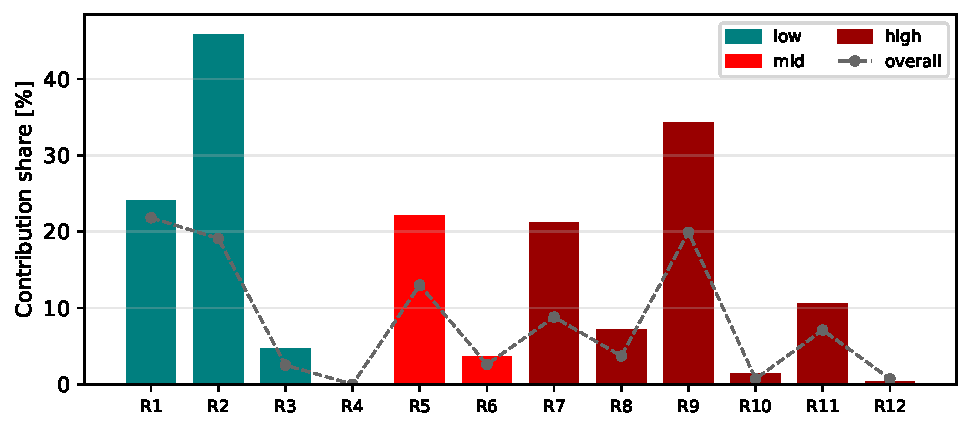
\includegraphics[width=\linewidth]{figures/rule_coverage.pdf}
  \caption{Contribution share of each rule to the fuzzy output: bars, within the records of the rule's own severity zone; dashed line, over all records. Colors follow the severity of the consequent.}
  \label{fig:coverage}
\end{figure}

\subsection{Membership functions and consequents}

Figure~\ref{fig:mfs} shows the interval membership functions of the two variables that appear most often in the rulebase and the linguistic partition of the output. Every transition crosses 0.5 exactly at a tree threshold, so the fuzzy partition remains traceable to the trees; the transition widths follow the training-data distribution inside each interval, with the sharpness factor selected in the inner folds. Figure~\ref{fig:singletons} presents the tuned consequent singletons: the least-squares adjustment spreads them inside their normative ranges without violating any boundary, and the six severe consequents grade the intervention range from 9.7 to 19.9 [mpy].

\begin{figure*}[htb!]
  \centering
  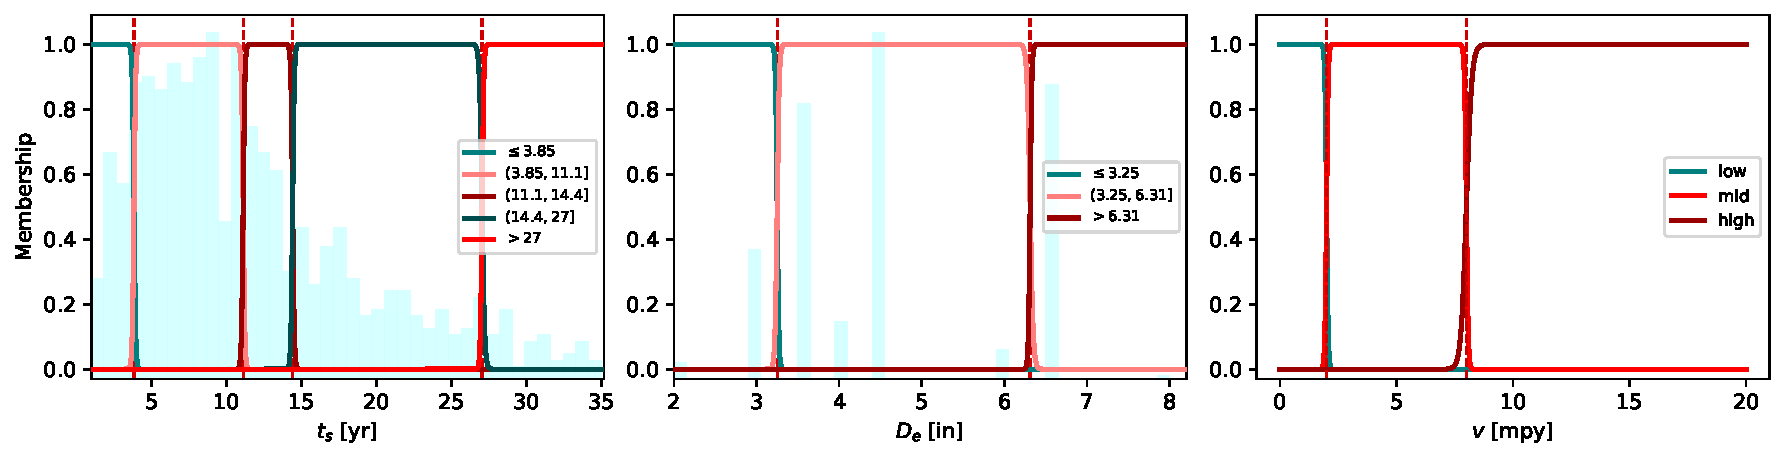
\includegraphics[width=\textwidth]{figures/mf_three_panel.pdf}
  \caption{Interval membership functions derived from the tree thresholds (dashed lines): (a) service time $t_s$, (b) external diameter $D_e$, with the training histograms in the background; (c) linguistic partition of the output variable at the normative limits.}
  \label{fig:mfs}
\end{figure*}

\begin{figure}[htb!]
  \centering
  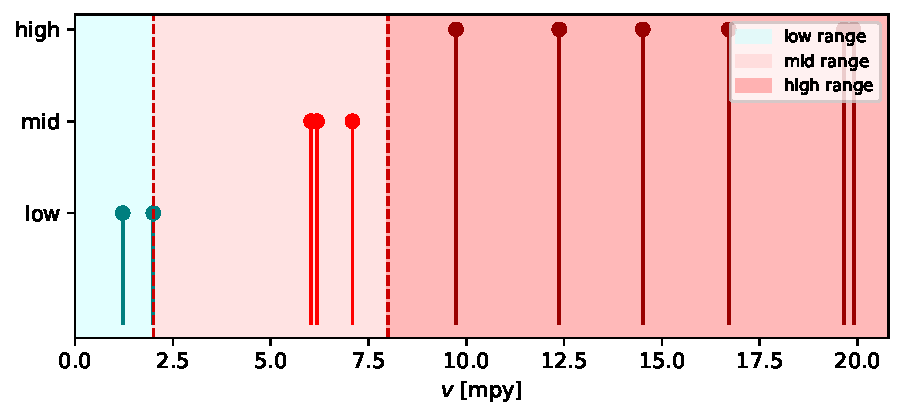
\includegraphics[width=\linewidth]{figures/consequent_singletons.pdf}
  \caption{Tuned consequent singletons of the twelve rules within the normative ranges (shaded). Dashed lines mark the 2 [mpy] and 8 [mpy] limits.}
  \label{fig:singletons}
\end{figure}

\subsection{Predictive performance}

The out-of-fold parity of the fuzzy system: an $R^2$ of 0.50, an MAE of 3.65 [mpy], and an RMSE of 5.20 [mpy] over the 897 records. Figure~\ref{fig:response} demonstrates the property promised by the formulation: sweeping the service time with the remaining variables at their medians produces a continuous output that ramps across the normative limits instead of jumping between class labels.

\begin{figure}[htb!]
  \centering
  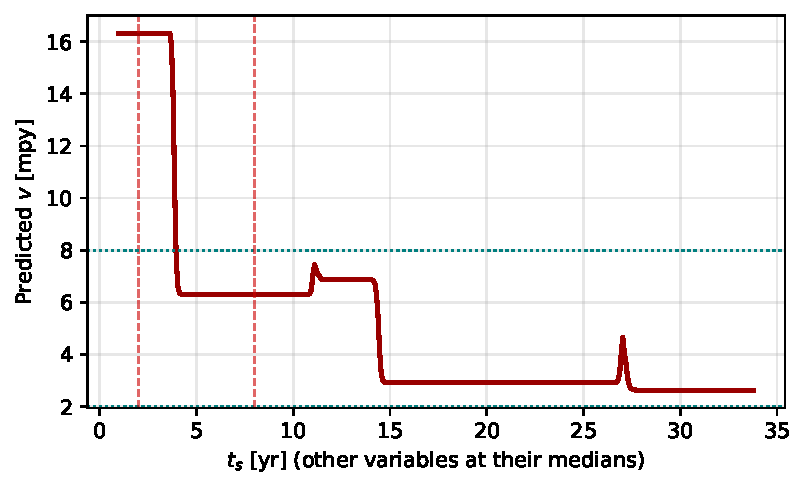
\includegraphics[width=0.9\linewidth]{figures/response_curve.pdf}
  \caption{Response of the fuzzy system to the service time with the remaining variables at their medians. The output ramps smoothly across the normative limits (dashed and dotted lines).}
  \label{fig:response}
\end{figure}

\subsection{Comparison on identical folds}

Table~\ref{tab:comparison} and Figure~\ref{fig:box} compare the four methods under the identical nested protocol, reporting the global out-of-fold value and the minimum--maximum band across the five outer folds. The fuzzy system reaches the lowest MAE after the decision-tree regressor (3.65 against 3.34 [mpy]) and surpasses linear regression (4.15 [mpy]) and support vector regression (3.82 [mpy]); its $R^2$ of 0.498 exceeds both (0.492 and 0.486) and remains within 0.04 units of the decision-tree regressor (0.540).

\begin{table}[htb!]
\centering
\footnotesize
\setlength{\tabcolsep}{4pt}
\caption{Out-of-fold comparison on identical folds: global value (min--max across the five outer folds).}
\label{tab:comparison}
\begin{tabular}{@{}lccc@{}}
\toprule
Method & MAE [mpy] & $R^2$ & Recall$_{high}$ \\
\midrule
\midrule
Proposed FIS & 3.65 (3.22--4.21) & 0.498 (0.38--0.60) & 0.78 \\
Linear reg. & 4.15 (3.87--4.47) & 0.492 (0.44--0.54) & 0.89 \\
Decision-tree reg. & 3.34 (2.99--3.79) & 0.540 (0.47--0.58) & 0.78 \\
SVR & 3.82 (3.43--4.26) & 0.486 (0.42--0.54) & 0.80 \\
\bottomrule
\end{tabular}
\end{table}


\begin{figure*}[htb!]
  \centering
  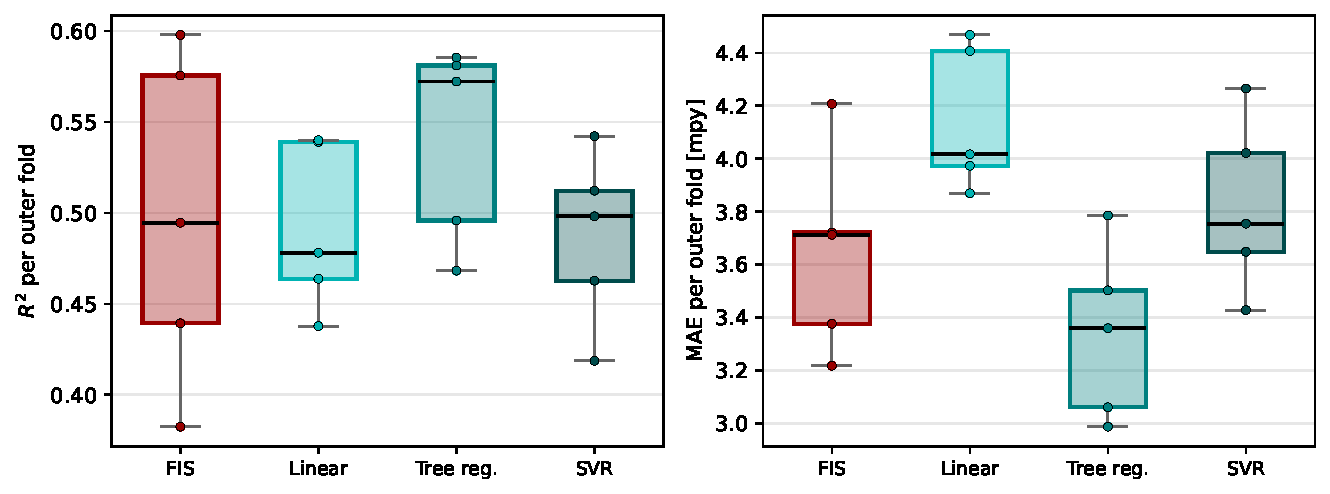
\includegraphics[width=0.92\textwidth]{figures/nested_boxplots.pdf}
  \caption{Per-fold distribution of $R^2$ and MAE for the four methods under the identical nested protocol (five outer folds; boxes span the interquartile range, whiskers the full min--max band, points mark the individual folds).}
  \label{fig:box}
\end{figure*}

Figure~\ref{fig:zones} decomposes the error by severity zone. The fuzzy system improves on linear regression in every zone (3.14 against 4.02 [mpy] in the low zone, 2.82 against 3.30 in the medium zone, and 4.66 against 4.94 in the high zone) and attains the lowest low-zone error of all four methods. Thresholding the continuous outputs at the normative limits shows why the strategy separates the classification and estimation roles: thresholded linear regression recovers the high class strongly (recall 0.89) only by overpredicting --- its low-class recall collapses to 0.31 --- whereas the dedicated classification layer of the strategy delivers balanced recalls (0.80 and 0.81 at the 8 [mpy] limit).

\begin{figure}[htb!]
  \centering
  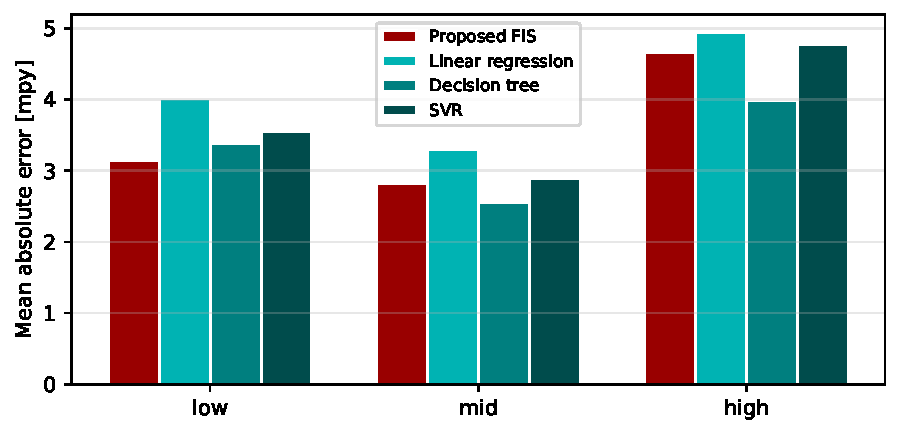
\includegraphics[width=\linewidth]{figures/error_by_zone.pdf}
  \caption{Mean absolute out-of-fold error by severity zone for the
    four methods.}
  \label{fig:zones}
\end{figure}

\subsection{Why the decision-tree regressor is less interpretable}

The decision-tree regressor offers the lowest global error, and a single tree is often presented as an interpretable model. Four structural facts separate it from the proposed system in this application.

First, its complexity: the trees selected by the inner loops carry between 15 and 45 leaves per fold. Each leaf is one disjoint rule, so the regressor speaks through 15--45 rules, against twelve rules with at most four conditions. An expert can audit twelve propositions; a forty-leaf partition exceeds the practical limit of rule-by-rule verification.

Second, its consequents: each leaf outputs the unconstrained mean of its training records. Nothing ties these constants to the normative classes --- a leaf mean can sit anywhere, and no boundary separates a ``monitoring'' leaf from an ``intervention'' leaf. The proposed system bounds every consequent to the normative range of its severity class, so each rule speaks the language of the standard.

Third, its output geometry: the prediction is piecewise constant. The estimate jumps discontinuously when a variable crosses a threshold and remains flat elsewhere, which contradicts the gradual character of the corrosion phenomenon. The fuzzy system produces the smooth, monotone transitions of Figure~\ref{fig:response}.

Fourth, its severity structure: the regressor optimizes a global error without any notion of the normative classes, and its induced classification is as unbalanced as that of the other regressors. The proposed strategy carries a dedicated classification layer designed for exactly that criterion.

The comparison therefore delimits the position of each method: the fuzzy system concedes 0.04 units of $R^2$ in exchange for a continuous output with smooth transitions, consequents bounded to the normative ranges, a balanced severity classification, and a twelve-rule inference chain in which every prediction traces to explicit, verifiable service and operating conditions.
